\section{Antenner för VHF/UHF/SHF}
\index{antenn!VHF}
\index{antenn!UHF}
\index{antenn!SHF}

\subsection{Allmänt}

Alla antenner fungerar efter samma principer.
Principerna för kortvågsantenner kan därför tillämpas även för antenner för
högre frekvenser.
Byggmåtten på en VHF/UHF-antenn är betydligt mindre än för en motsvarande
HF-antenn.
Då våglängden \(\lambda\) vid 145~MHz är ca 2~m jämfört med ca 80~m vid 3,5~MHz
är möjligt att bygga riktantenner med rimliga dimensioner för VHF/UHF, även om
många antennelement används.

Om man bortser från rundstrålande vertikalantenner för trafik på korta avstånd
och mobil trafik, så används riktantenner främst på grund av den större
räckvidden.
En riktantenns egenskaper uttrycks i första hand i storheterna strålningsvinkel,
antennvinst, fram/backförhållande och halvvärdesbredd.

Eftersom polarisationsvridning sällan förekommer vid högre frekvenser, är det
viktigt att sändar- och mottagarantenner har samma polarisationsriktning.
Horisontell polarisation anses vara bättre lämpad för långa distanser, eftersom
vågor med horisontell polarisation böjer av bättre över horisontella
formationer (bergryggar etc).
Även passage genom skogspartier går bättre med horisontellt polariserade vågor.
Antenner med horisontell polarisation används därför ofta för SSB- och
CW-trafik på långa avstånd och utmed markytan.
Sådan trafik sker i allmänhet från fasta stationer.

För både mobil trafik och lokal fast trafik används oftast antenner med vertikal
polarisation.
Vertikala antenner ger de önskvärda rundstrålande egenskaperna för mobil trafik
och är bäst lämpade att montera på fordon.

\subsection{Riktantenner}
\index{antenn!riktantenn}
\index{riktantenn!elementlängd}
\label{riktantenn}

En \(\lambda/2\)-antenn strålar vinkelrätt ut från antennledaren och
runt omkring den.
Placeras ett reflektorelement (längd \(\approx\lambda/2 + 5\%\)) bakom antennen
på ett avstånd av \(\approx \lambda/5\) så reflekteras den bakåtriktade
strålningen delvis framåt.
En större del av energin kommer då att samlas i en riktning.
Med ett direktorelement (längd \(\approx\lambda/2 - 5\%\)) framför det
strålande elementet på ett avstånd av \(\approx\lambda/10\) så kommer
utstrålningsvinkeln att bli mindre.

\subsection{Yagiantenner}
\index{yagiantenn}
\index{antenn!yagi}

\begin{figure}
  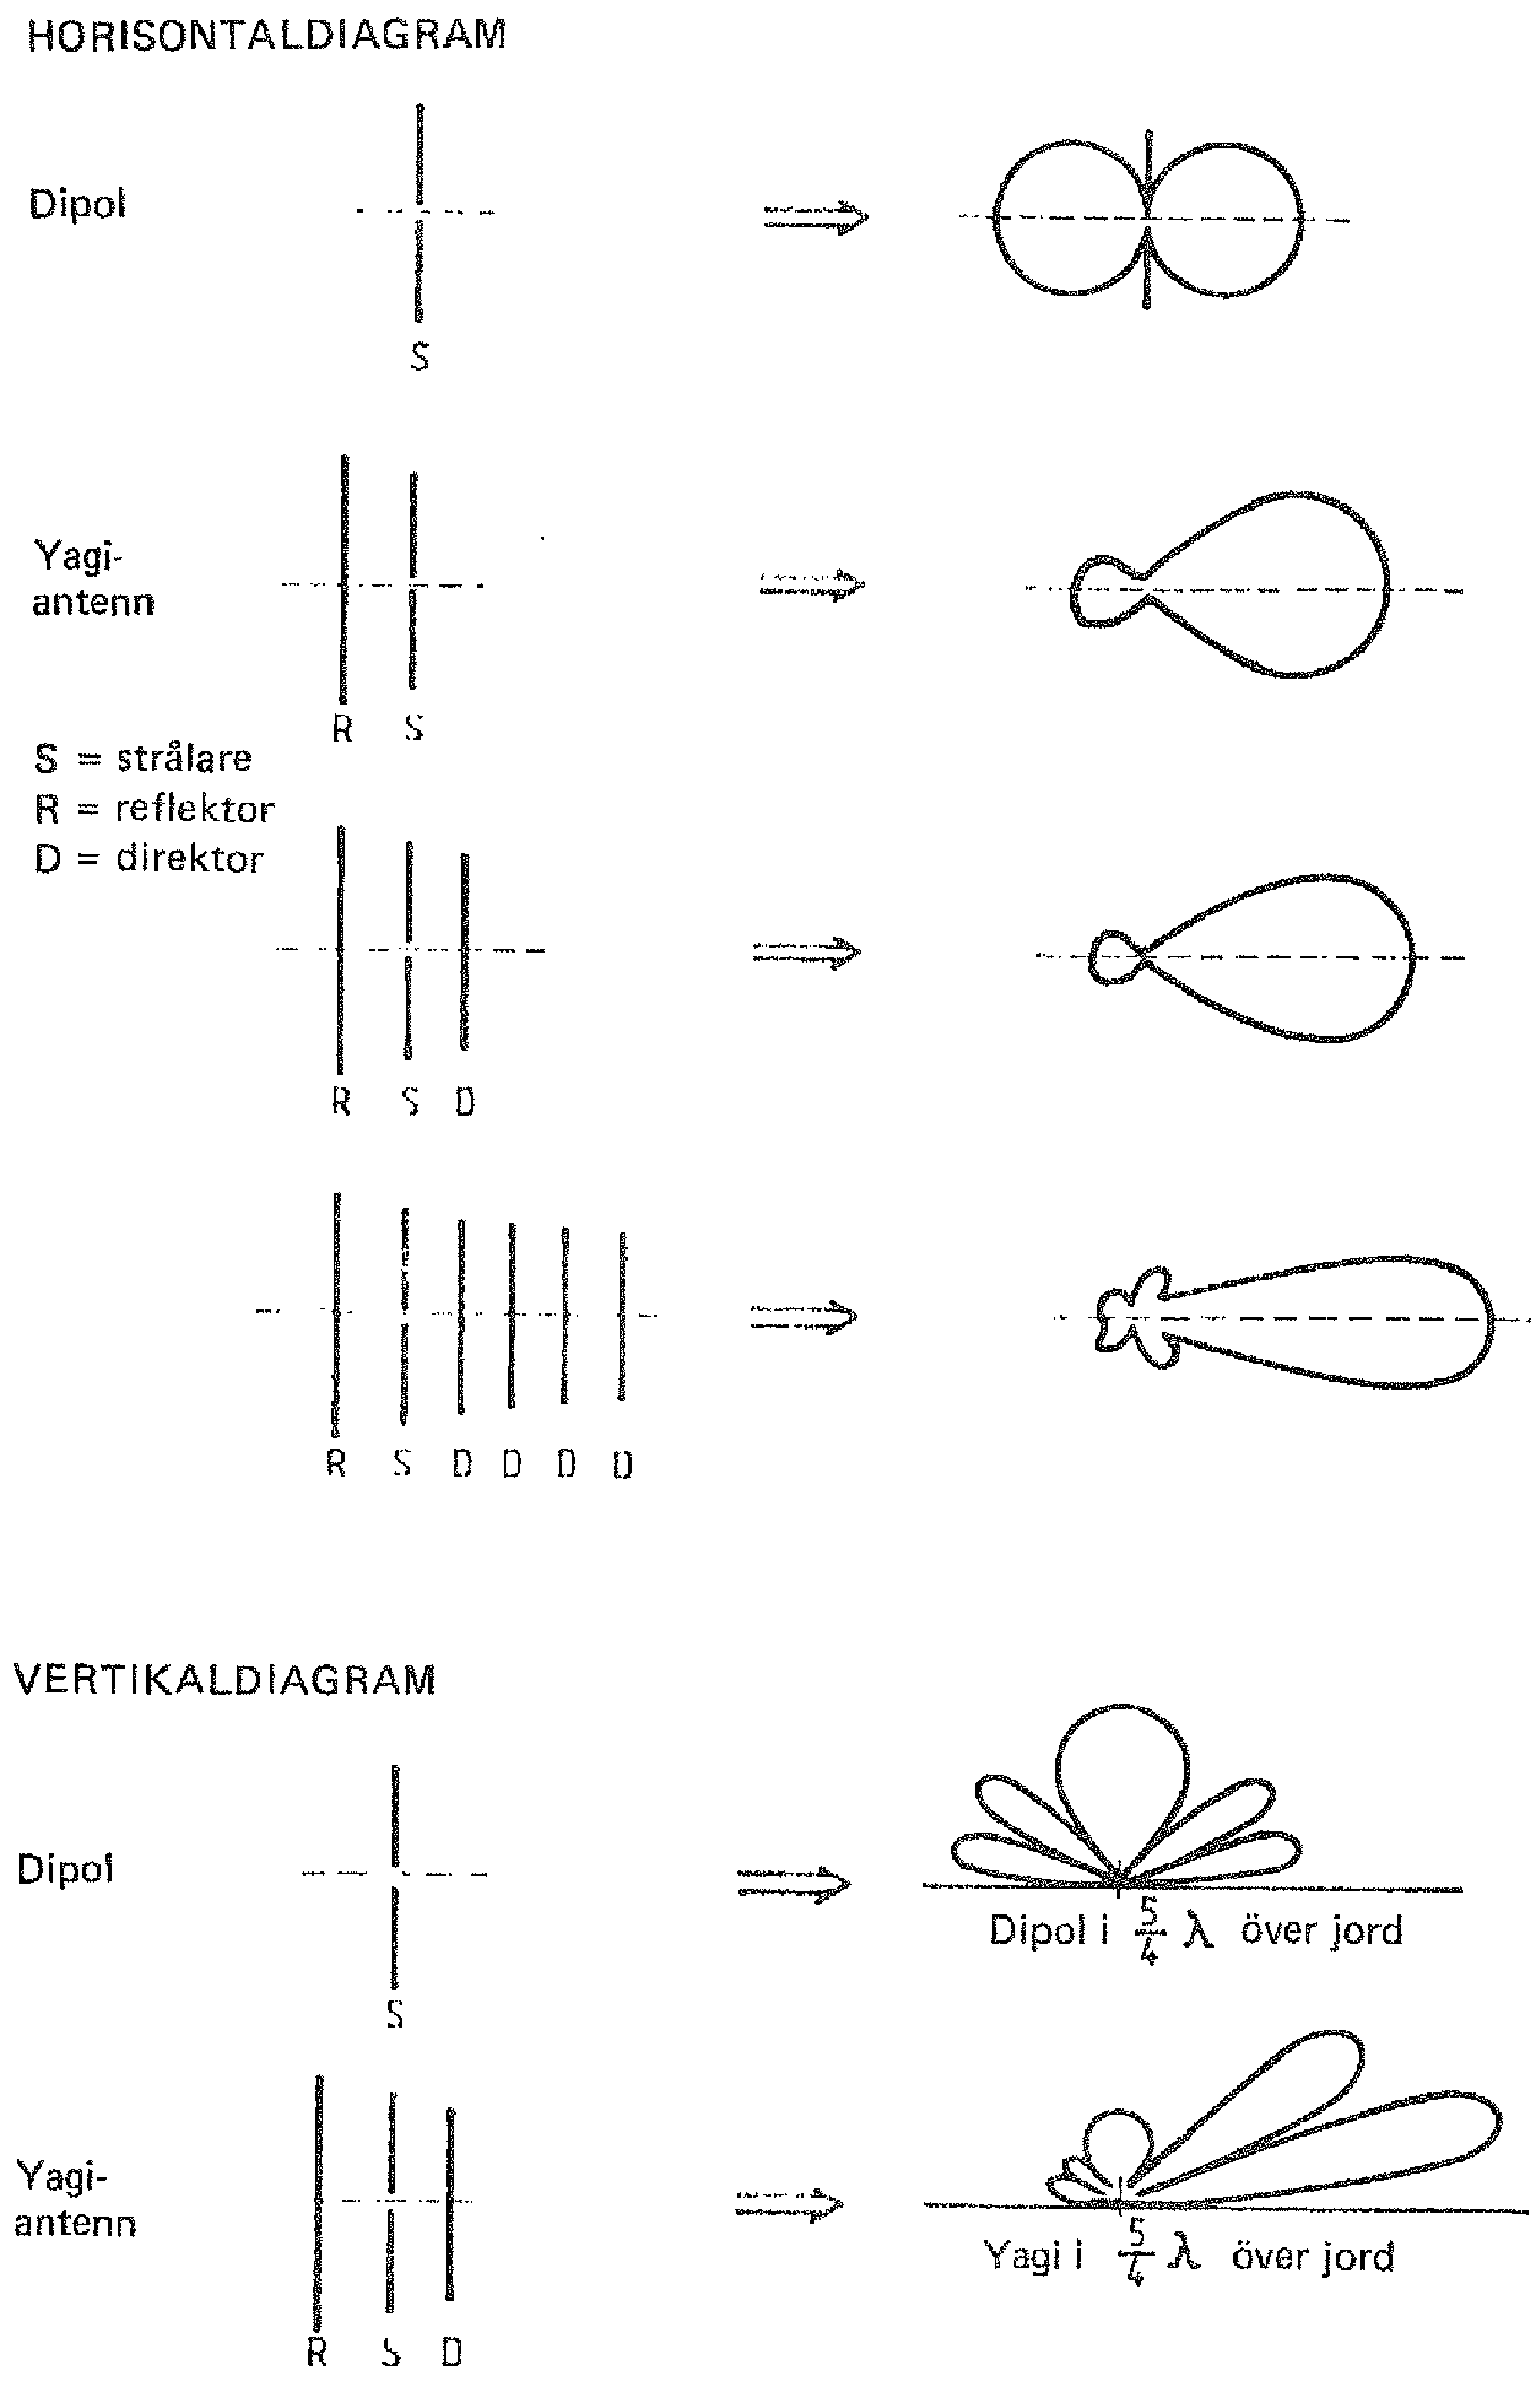
\includegraphics[width=\textwidth]{images/cropped_pdfs/bild_2_6-20.pdf}
  \caption{Strålningsdiagram för horisontell yagiantenn}
  \label{fig:bildII6-20}
\end{figure}

Den typ av riktantenn, som består av en strålare, en passiv reflektor
samt ett antal passiva direktorer, kallas \emph{yagiantenn} och illustreras i
bild \ref{fig:bildII6-20}.
Observera att vertikaldiagrammet visar strålningsdiagrammet med antennen
placerad nära jord.
För VHF, UHF och SHF placeras antennen ofta så högt över mark att antennen kan ses
som placerad i fri rymd.
Strålningsdiagrammet blir då annorlunda genom att antennens huvudlob sänks jämfört
med det i bilden och hamnar med centrum symmetriskt runt horisontalplanet.

Yagiantennen kan utföras med olika antal direktorelement i kombination med
olika längd.

Det finns tre sätt att optimera en riktantenn, nämligen maximal
riktverkan, minimala sidolober eller maximalt fram/backförhållande.
Dessa egenskaper är, emellertid ej möjliga att uppnå samtidigt.
Ökas till exempel antalet element, så ökar den så kallade antennvinsten genom
att öppningsvinkeln på strålningen blir mindre, men samtidigt minskar
matningsimpedansen och den användbara bandbredden.

Som tumregel kan man konstatera att det är inte mängden element som
avgör antennvinsten, utan den dominerande faktorn är längden på bommen.
Mängden element påverkar antennvinsten med 1--2~dB från optimal till
medioker.
Egenskaper som fram/back förhållande eller minimala sidolober beror mer
på mängden, placering och storlek på direktorerna.

\subsection{Gruppantenner}

Ordnas flera riktantenner vid sidan av och/eller över varandra så
erhålls en så kallad gruppantenn.
Ett sådant arrangemang av så kallade stackade antenner ger en ännu mindre
öppningsvinkel på strålningen vertikalt och/eller horisontellt.
Därigenom erhålls ytterligare antennvinst.

\subsection{Parabolantenner}
\textbf{
HAREC a.\ref{HAREC.a.6.1.6}\label{myHAREC.a.6.1.6}
}
\index{parabolantenn}
\index{antenn!parabol}
\index{antenn!SHF}

Särskilt på frekvenser i mikrovågsområdet och högre har radiovågorna i
stort sett samma utbredningsegenskaper som ljusets.
Behöver stor riktverkan uppnås på dessa höga frekvenser, används ofta en
parabolisk yta som spegel bakom själva antennen, tillsammans kallas det dock
för \emph{parabolantenn}.
Jämför med reflektorn i en ficklampa.

Den egentliga antennen (den s.k. mataren), vars strålning är riktad
mot parabolen för att reflekteras, kan vara utformad på många sätt.
Eftersom parabolens storlek står i omvänd proportion till frekvensen, så
används av praktiska skäl inte paraboliska reflektorer på låga frekvenser.

\subsection{Övriga antenntyper}

Rundstrålande antenner: Ground plane, \(\lambda/4\)-, \(\lambda/2\)-,
\(5\lambda/8\)-antenner m.fl.

Riktantenner: Quad-, HB9CV-, helical-, parabol- och hornantenner med flera.
